\documentclass[utf8]{ctexart}
\usepackage{amsrefs}
\usepackage{amsmath}
\usepackage{amssymb}
\usepackage{geometry}
\usepackage{graphicx}
\usepackage{float}  %设置图片浮动位置的宏包
\usepackage{subfigure}%插入多图时用子图显示的宏包
\title{Assignment1}
\author{ZuoXichen-2000012103}
\begin{document}
    \maketitle
    \paragraph*{第一题}重量法、库仑法、凝固点下降法、称量滴定法和同位素稀释质谱法。
    \paragraph*{第二题}正态分布是最一般的分布,u分布是正态分布的0, 1标准化形式,而t分布则用于较小样本的分布,当样本数n趋于无穷时,t分布则趋于正态分布。
    \paragraph*{第三题}39.0983*2+51.9961*2+15.9994*7=242.1885
    \paragraph*{第四题}
    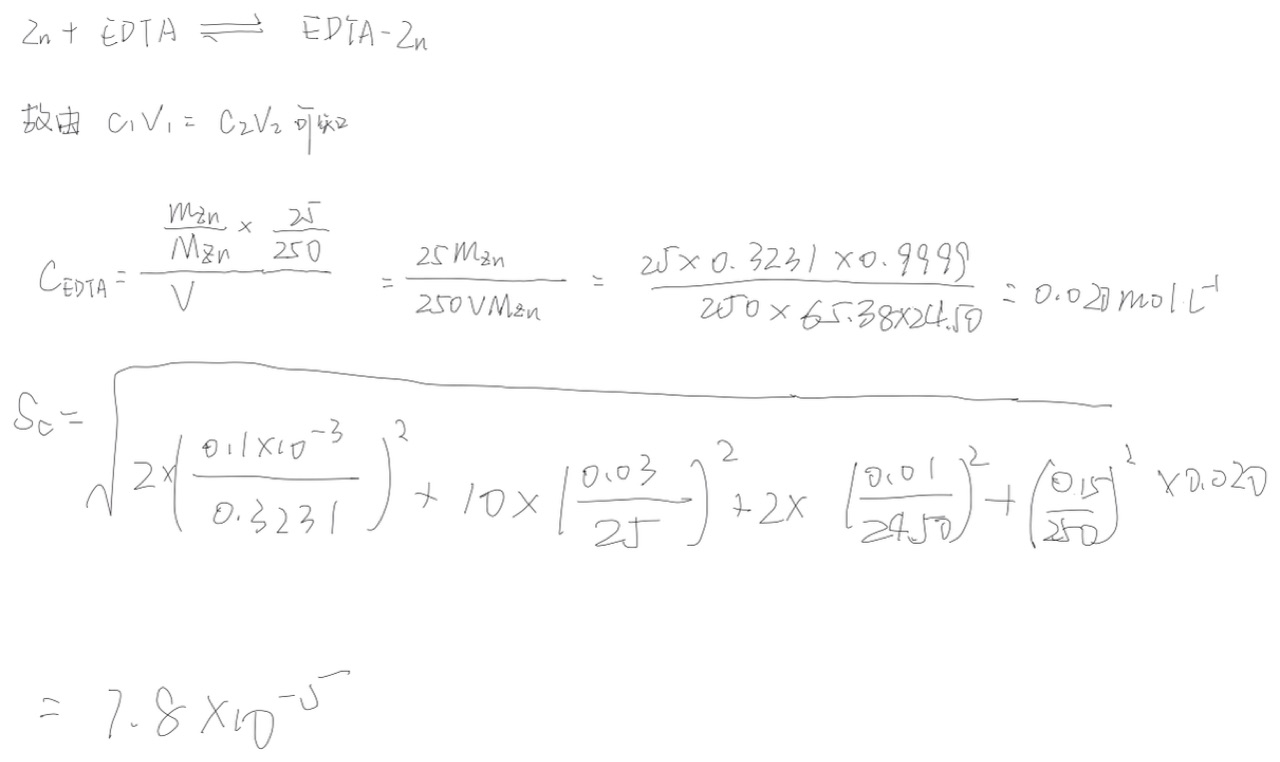
\includegraphics[scale=0.3]{lib/assign1-1.jpg}
    \paragraph*{第五题}
    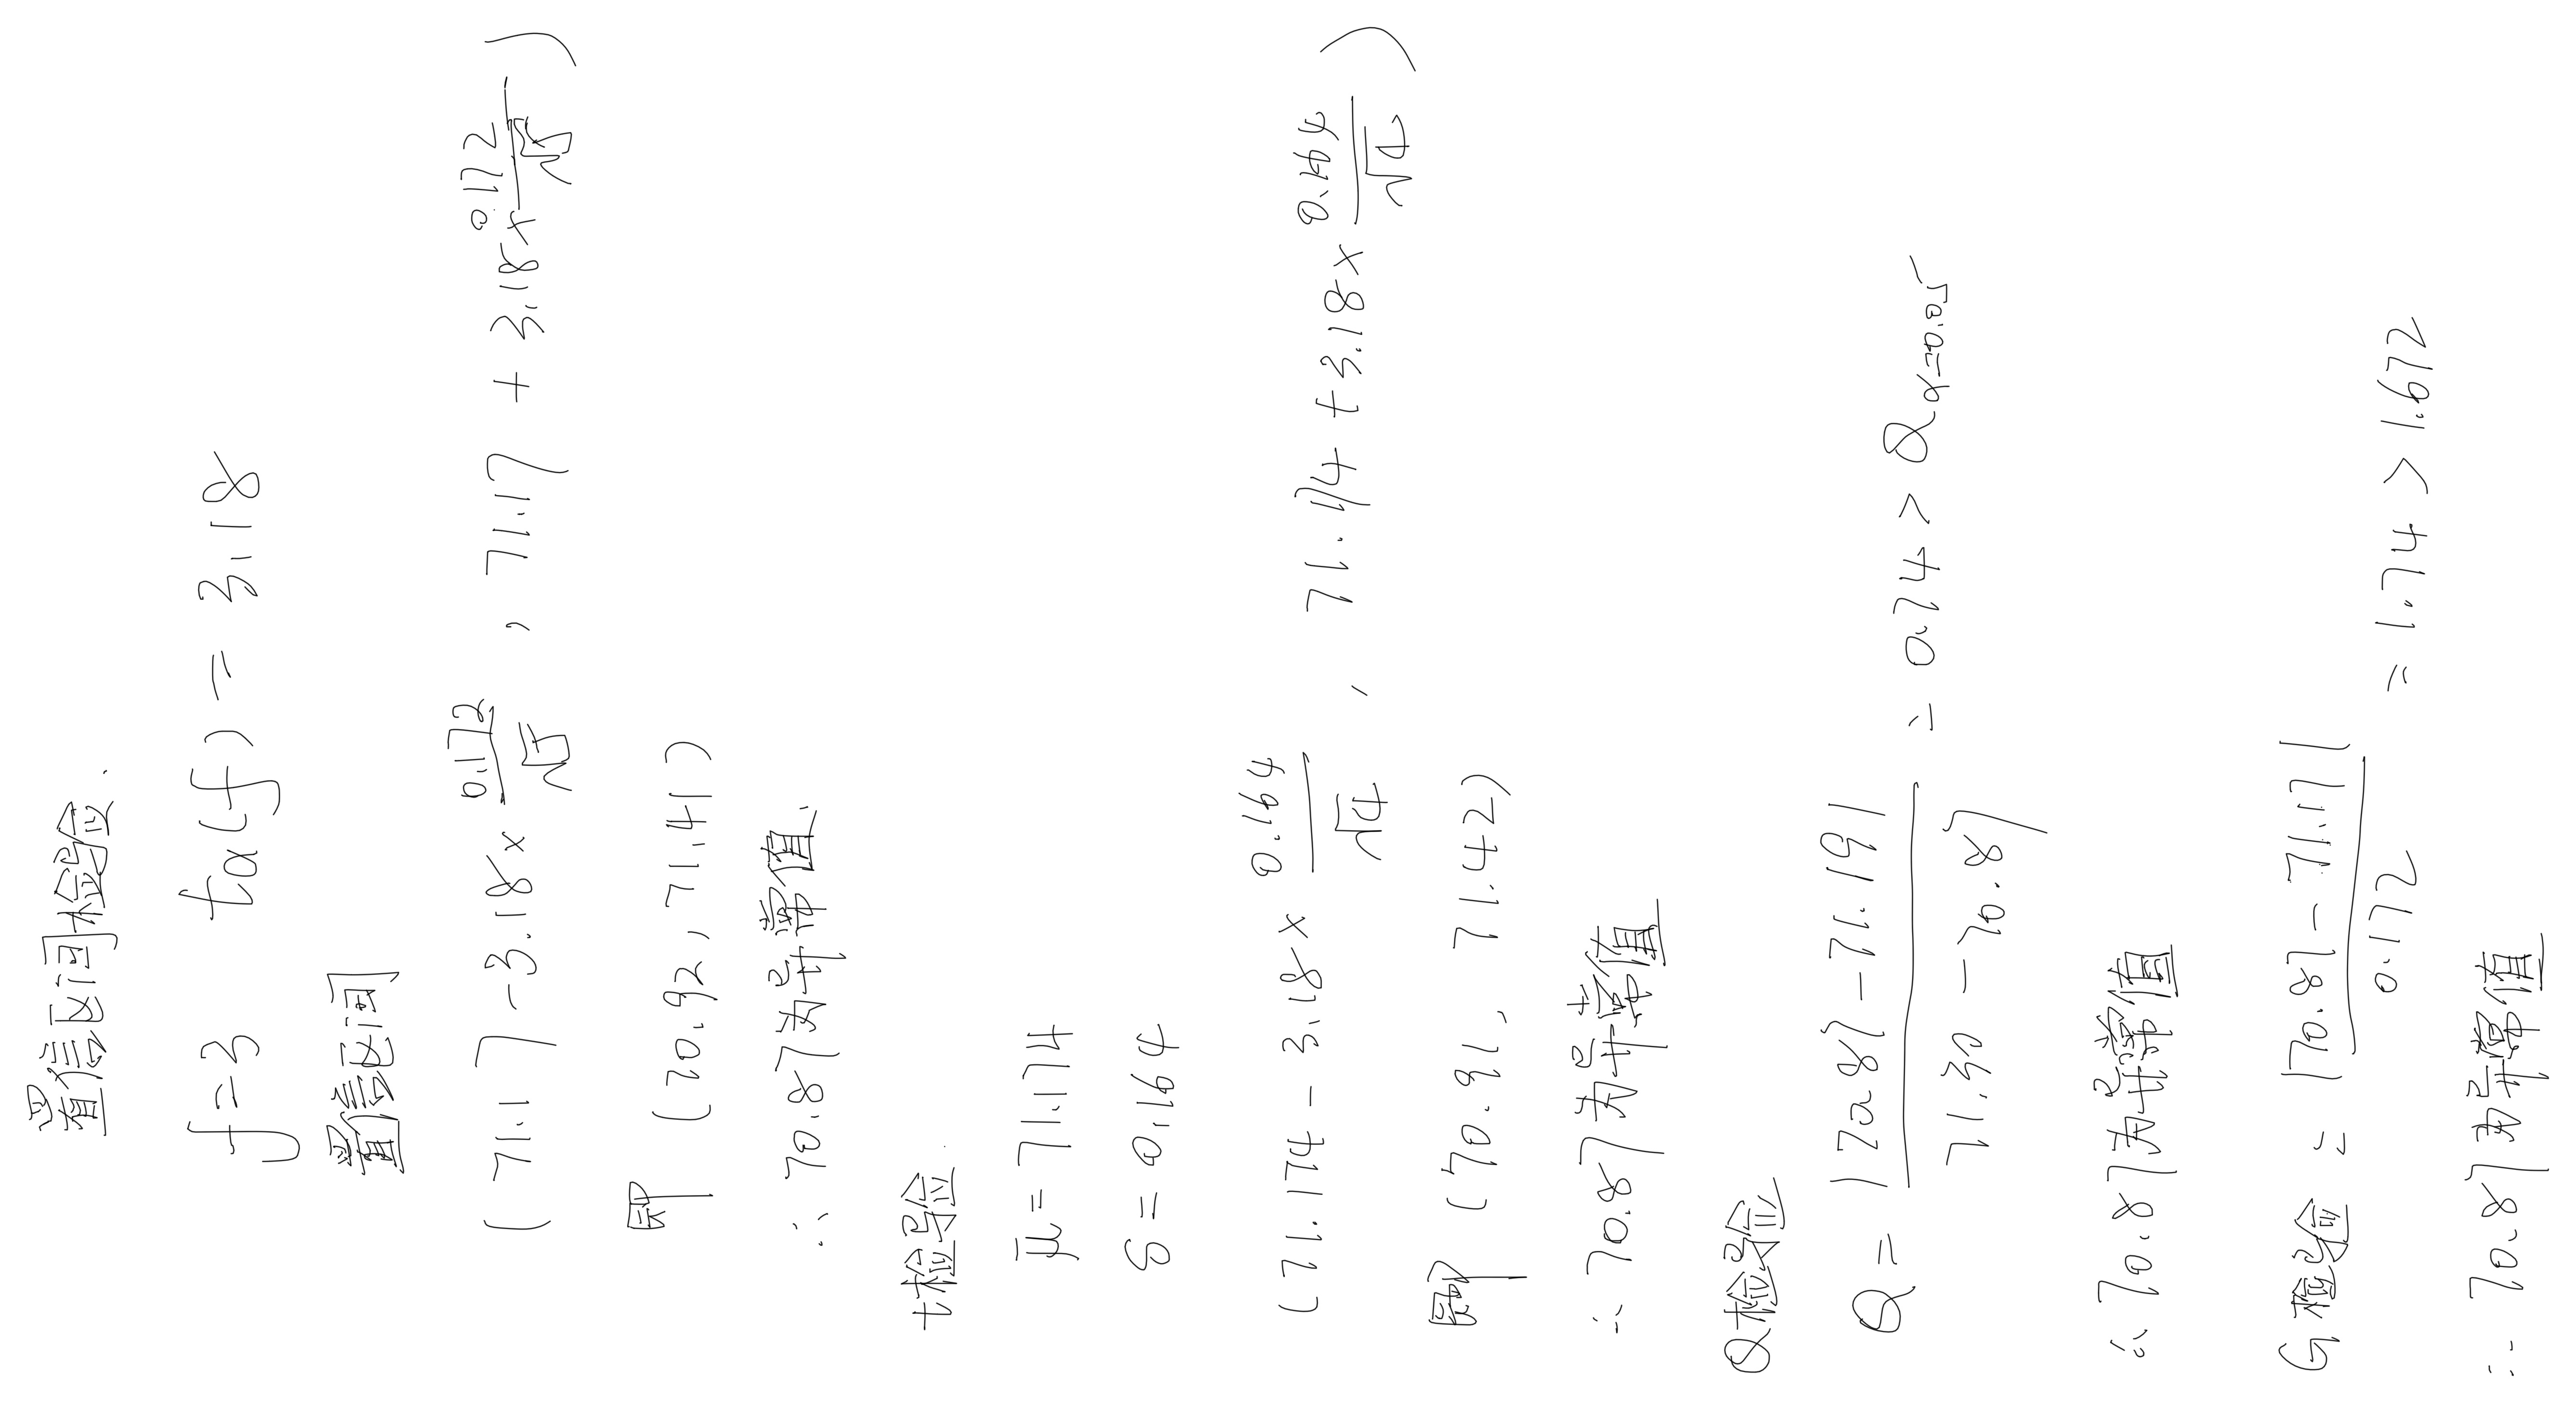
\includegraphics[scale=0.6]{lib/assign1-2.jpg}
\end{document}